\documentclass[
../../EiKI_Summary.tex,
]
{subfiles}
    
\externaldocument[ext:]{../../EiKI_Summary.tex}
% Set Graphics Path, so pictures load correctly
\graphicspath{{../../}}

\begin{document}
\section{Machine Learning \& Neural Networks}
\subsection{Learning}
Learning is an essential process for dealing with unknown environments. An agent is almost \defc{never omnisicient}.

Learning also makes an agent ''aware'' of their environment. Rather than trying to change the environment so that they can take their actions, they might \defc{try to use and adapt to the environment} to fulfill their tasks.

Lastly, Learning improves the agents decision mechanisms the longer it is active. No longer will an agent repeat actions hoping for different results (e.g. local extrema).

\subsubsection{Methods of Learning}
\defc{Memorization (Declarative Knowledge):}\\
Accumulates individual facts and their outcomes. This is limited by the time to observe facts and memory to store facts.

Better: \defc{Generalization (Imperative Knowledge):}\\
Deduce new facts from old facts. Limited by accuracy of deduction process, assumes relations between past and future.

\subsubsection{Inductive Learning}
Inductive learning is the simplest form of learning. It deduces a trend from examples.

\textbf{Basic Idea:}
\begin{itemize}
    \item $f$ is the (unknown) target function. $f(x)$ is then called the target
    \item Examples are defined in the form $(x,f(x))$ e.g. Weather data: (1, Rain)
    \item Use examples to find a hypothesis $h$ such that $h \approx f$
\end{itemize}

Hypothesis $h$ is \defc{consistent} if \inlmathbox{$\forall x: h(x) = f(x)$}.

\begin{minipage}
    [t]{0.5\textwidth}
    \begin{defbox}
        [Ockhams Razor]
        The \defc{best explanation} is the \defc{simplest explanation} that fits the data
    \end{defbox}
\end{minipage}
\begin{minipage}
    [t]{0.5\textwidth}
    \begin{defbox}
        [Overfitting Avoidance]
        Maximize the combination of consistency and simplicity.
    \end{defbox}
\end{minipage}

\subsection{Machine Learning}
Programming an algorithm to automatically learn a program from data or experience.

Machine Learning is \defc{not synonymous} with AI. Many AI algorithms are based on Machine Learning, but not all. 

\subsubsection{Machine Learning \& Human Learning}
Human learning is often
\begin{itemize}
    \item very data- and knowledge efficient
    \item a complete multitasking, multi-modal system
    \item time-inefficient
\end{itemize}

Machine learning is often inspired by human learning, the goal however, is not to recreate human learning.
\begin{itemize}
    \item May borrow idead from human learning (e.g. neural networks)
    \item May perform better or worse
\end{itemize}

\subsubsection{Designing a Learning System}
\defc{Machine Learning is not the solution to every problem!}

\begin{enumerate}
    \item Do I need a learning approach for my problem?
    \begin{itemize}
        \item Is there a pattern to detect?
        \item Can I solve the problem analytically?
        \item Do I have data to train on?
    \end{itemize}
    \item What type of problem do we have?
    \begin{itemize}
        \item How to represent it?
        \item Which algorithm to use?
    \end{itemize}
    \item Gather and organize data
    \begin{itemize}
        \item Preprocessing is important
    \end{itemize}
    \item Fitting / Training your model
    \item Optimization
    \item Evaluate and iterate back to step 2
\end{enumerate}

\subsubsection{Types of Learning}
\begin{defbox}
    [Supervised Learning]
    Learning based on labeled datasets. Learns to map inputs to outputs based on pairs in the dataset.
\end{defbox}

\begin{defbox}
    [Unsupervised Learning]
    Learning based on unlabeled datasets. Searches for patterns and similarities in the data.
\end{defbox}

\begin{defbox}
    [Reinforcement Learning]
    Agent acts and receives positive or negative reward. The agent learns to act in a way that maximizes the reward.
\end{defbox}

\newpage
\subsubsection{Supervised Learning}
\defc{Given:} Dataset $(x_1,y_1), \ldots, (x_n,y_n)$

\defc{Goal:} Find a function $h$ such that $h(x_i) \approx y_i$

\begin{minipage}
    [t]{0.5\textwidth}
    \begin{defbox}
        [Regression Task]
        \begin{itemize}
            \item y is a continous value
            \item Example: Temperature tomorrow
        \end{itemize}

        \begin{center}
            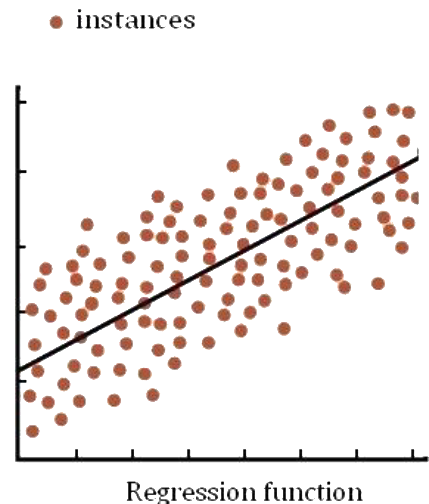
\includegraphics[width=0.5\textwidth]{Pics/11/RegressionFunction.png}
        \end{center}
    \end{defbox}
\end{minipage}
\begin{minipage}
    [t]{0.5\textwidth}
    \begin{defbox}
        [Classification Task]
        \begin{itemize}
            \item y is a discrete class label
            \item Algorithm tries to predict a continous value describing the label probability
            \item Example: Will it be above 0\degree C tomorrow?
        \end{itemize}

        \begin{center}
            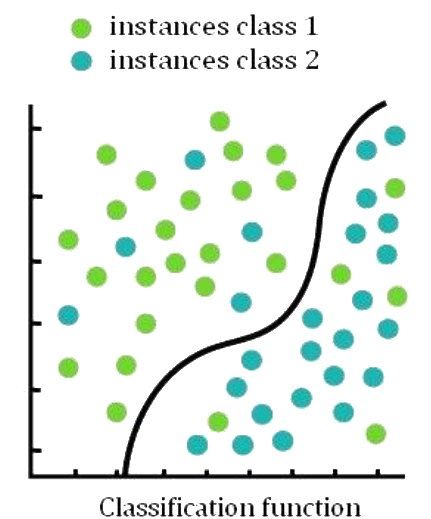
\includegraphics[width=0.5\textwidth]{Pics/11/ClassificationFunction.png}
        \end{center}
    \end{defbox}
\end{minipage}

\subsubsection{Representation}
Machine learning algorithms need to handle a lot of different data (e.g. images, audio, etc.). 

To make this as easy as possible we represent out input as an \defc{input vector} (in $\mathbb{R}^n$). Vectors are a great representation as we can transform the data using linear algebra. 

\begin{defbox}
    [Representation]
    Mapping input to another space, that is \defc{easier} to manipulate.
\end{defbox}

\begin{defbox}
    [Feature]
    Features are the \defc{independent variables} in machine learning models.
\end{defbox}

\begin{defbox}
    [Model]
    The representation of what our algorithm has learned from the data it used in training. The model is the \defc{output representation } of the learned ''rule set''.
\end{defbox}

\subsubsection{Feature Engineering}
Feature engineering is the process of selecting, manipulating and transforming raw data into features that can be used for machine learning.

For this it is important to know your data:
\begin{itemize}
    \item Data distribution
    \item Outliers
    \item Data reflective of reality
    \item Biased data
    \item \dots
\end{itemize}

On the basis of these factors we can choose approches that best fit our needs.

\begin{minipage}
    [t]{0.5\textwidth}
    \defc{Regression:}
    \begin{itemize}
        \item Linear Regression
        \item Multiple Linear Regression
        \item Regression Trees
        \item Non-linear Regression
        \item Polynomial Regression
        \item \dots
    \end{itemize}
\end{minipage}
\begin{minipage}
    [t]{0.5\textwidth}
    \defc{Classification:}
    \begin{itemize}
        \item Random Forest
        \item Decision Trees
        \item Logistic Regression
        \item Na\"ive Bayes
        \item Support Vector Machines
        \item \dots
    \end{itemize}
\end{minipage}

\subsection{Evaluating a Model}
To evaluate a model we need to know the goal we are trying to achieve.

Based on the goal we can use different evaluation metrics. These are the most common ones:
\begin{itemize}
    \item Accuracy
    \item Precision
    \item Recall
    \item Mean Squared Error
    \item \dots
\end{itemize}

Which metric is best depends on the problem we are trying to solve.

\subsubsection{Overfitting}
Overfitting describes the problem, that a model is trained ''too well'' so that its closer to memorization than generalization. This means that the model is not able to generalize to new data and therefore performs worse on new data.

To deal with overfitting we can:
\begin{itemize}
    \item Splitting data
    \begin{itemize}
        \item Split data into training and test data  
    \end{itemize}
\end{itemize}
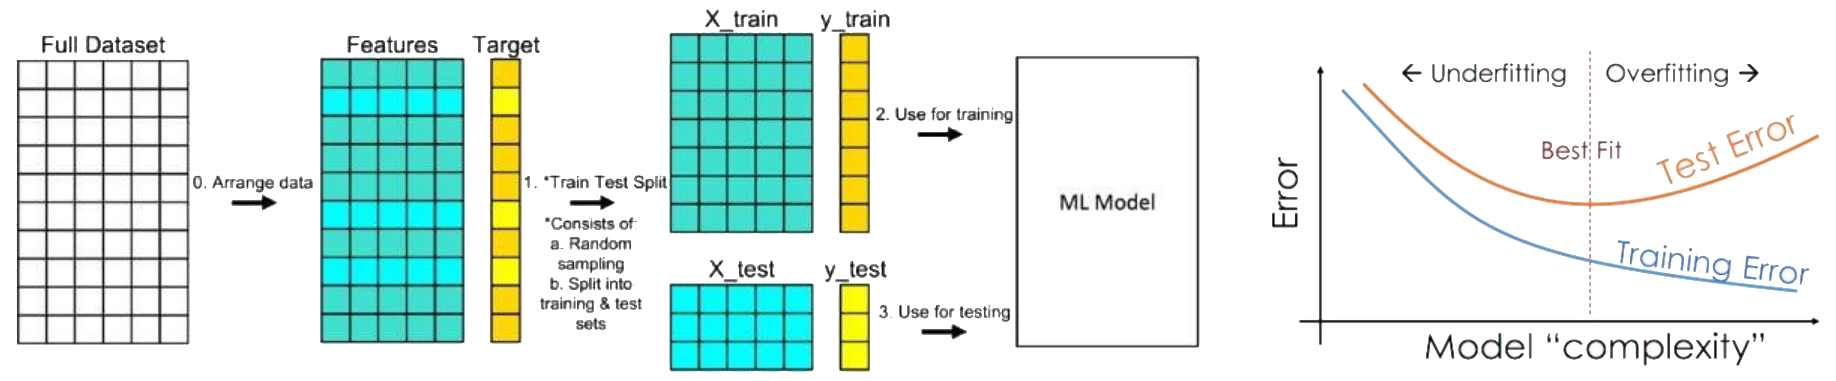
\includegraphics[width=\textwidth]{Pics/11/SplittingData.png}

\begin{itemize}
    \item Regularization 
    \item Use more data, augement data (adding noise)
    \item Select different features
    \item Cross validation
    \item Ensemble methods
\end{itemize}

\newpage
\subsection{Neural Networks}
\subsubsection{Deep Learning}
Up until now we always had to supervise learning in some way, like feature extraction. 

But with deep learning we can \defc{learn the underlying features} directly from data without specifying them.

\subsubsection{Perceptron}
The perceptron can be seen as an \defc{artificial neuron}. It takes multiple inputs, that are weighed individually and summed up to give a single output.

\begin{figure}
    [H]
    \centering
    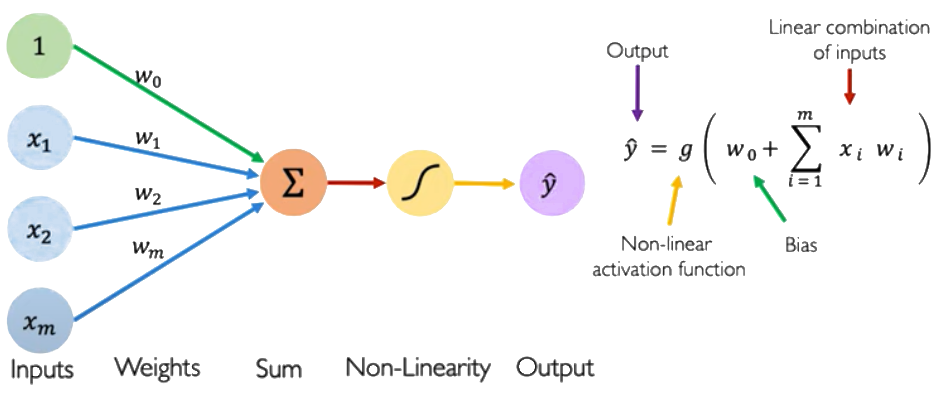
\includegraphics[width=0.9\textwidth]{Pics/11/Perceptron.png}
\end{figure}

\begin{itemize}
    \item Neurons correspond to nodes or units
    \item A link from unit j to uni i propagates activation y from j to i
    \item The weight $w_{i,j}$ of the link determines the strength and sign of the connection
    \item All weights together are called W or $\theta$ and describe the model
    \item The \defc{total input activation} is the sum of the input activations
    \item The \defc{output activation} is determined by the activation function g
\end{itemize}

\begin{defbox}
    [Activation Function]
    A activation function decides if a neuron should be active. Nowadays they're mostly non-linear.

    \begin{center}
        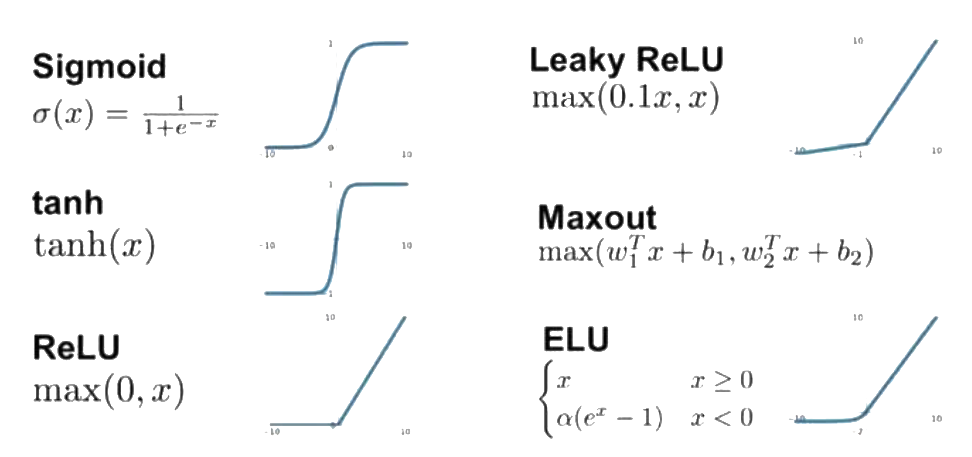
\includegraphics[width=0.5\textwidth]{Pics/11/ActivationFunction.png}
    \end{center}

    \begin{minipage}
        [c]{0.5\textwidth}
        \textbf{Why do we need an activation function?}
        \begin{itemize}
            \item It adds non-linearity to a neural network
            \item Without it we would have a linear regression model
            \item Allows for backpropagation
        \end{itemize}
    \end{minipage}
    \begin{minipage}
        [c]{0.5\textwidth}
        \centering
        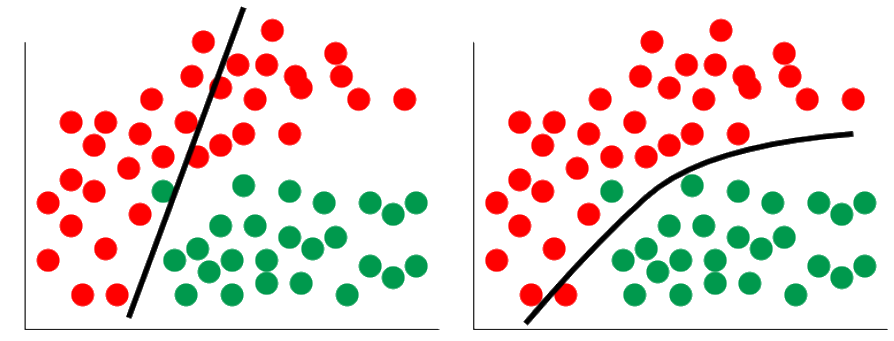
\includegraphics[width=0.8\textwidth]{Pics/11/Linear_NonLinear.png}
    \end{minipage}
\end{defbox}

\subsubsection{Perceptron to Neural Network}
\begin{minipage}
    [t]{0.4\textwidth}
    \begin{itemize}
        \item Perceptrons may have multiple output nodes which can be combined to other perceptrons
        \item We can build networks of these node: \defc{Multilayer Perceptron (MLP)}
        \item In a MLP information flow is \defc{unidirectional}
        \item Information is distributed and processed in parallel
        \item For each node:\\ \inlmathbox{$z_{k,i} = \sigma(w_{0,i}^k + \sum_{j=1}^{n_{k-1}} z_{k-1,j}\cdot w_{j,i}^k)$}
    \end{itemize}
\end{minipage}
\begin{minipage}
    [t]{0.6\textwidth}
    \begin{center}
        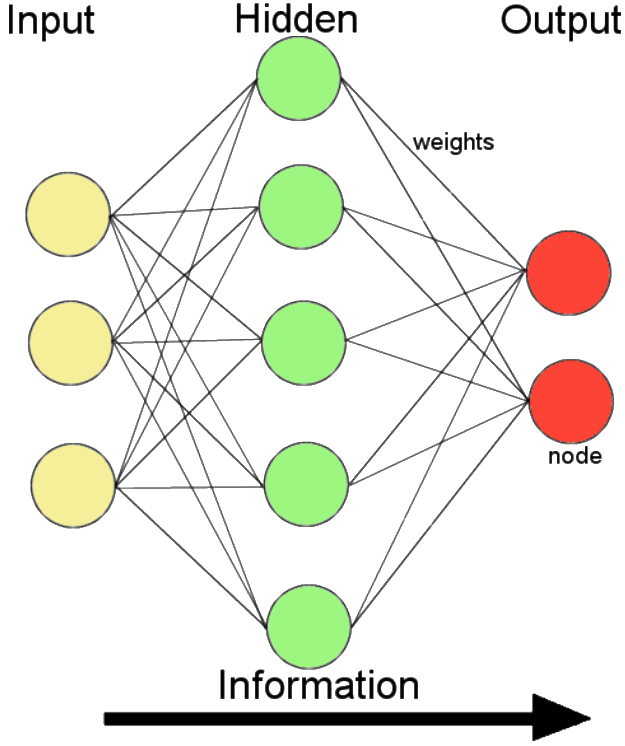
\includegraphics[valign=T,width=0.6\textwidth]{Pics/11/MLP.png}
    \end{center}
\end{minipage}

\subsection{Forward Propagation}
\subsubsection{Applying a NN}
Assume a distribution of an exam:

\begin{minipage}
    [t]{0.5\textwidth}
    \centering
    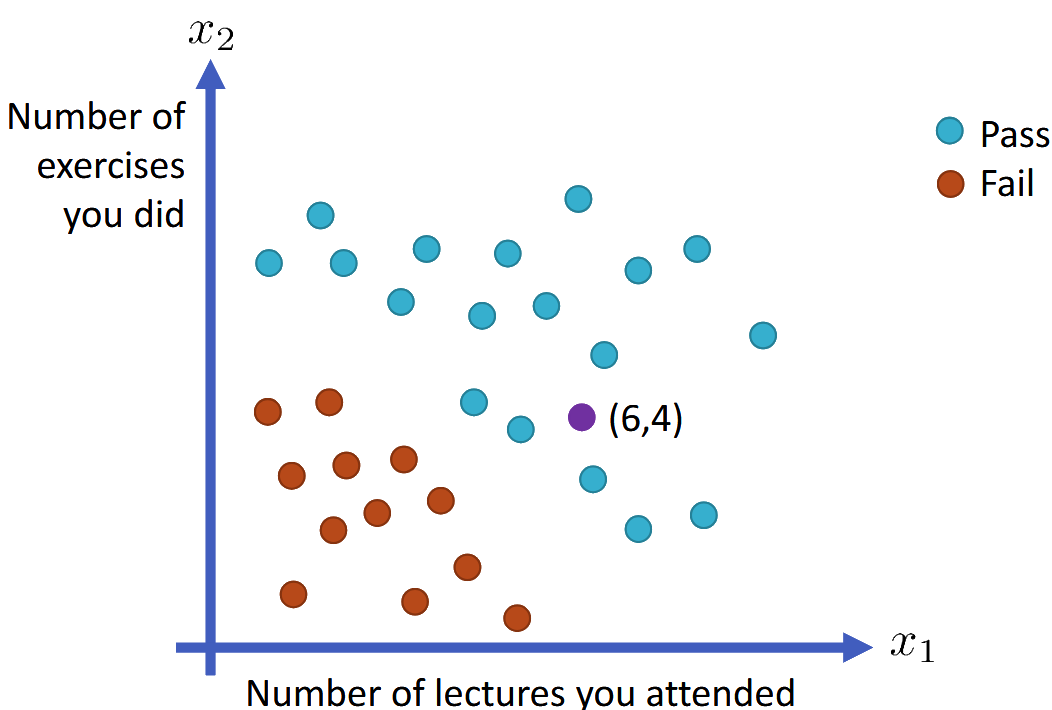
\includegraphics[valign=T,width=0.7\textwidth]{Pics/11/PredictionExample.png}
\end{minipage}
\begin{minipage}
    [t]{0.5\textwidth}
    Assume the purple point is $x_1 = 6, x_2 = 4$ and the weights of our NN are:

    \begin{csmb*}
        $\begin{array}{l l l}
            w_{1,1}^1 = 0.5 & w_{2,1}^1 = -1 & w_{1,1}^2 = -1 \\
            w_{1,2}^1 = 0.\overline{33} & w_{2,2}^1 = 0.5 & w_{2,1}^2 = -0.8 \\
            w_{1,3}^1 = 0.1 & w_{2,3}^1 = 0.6 & w_{3,1}^2 = 2 \\
        \end{array}$
    \end{csmb*}

    Further assumme a bias $w_{0,i}^k = 0$.
\end{minipage}

This yields a NN model:

\begin{figure}[H]
    \centering
    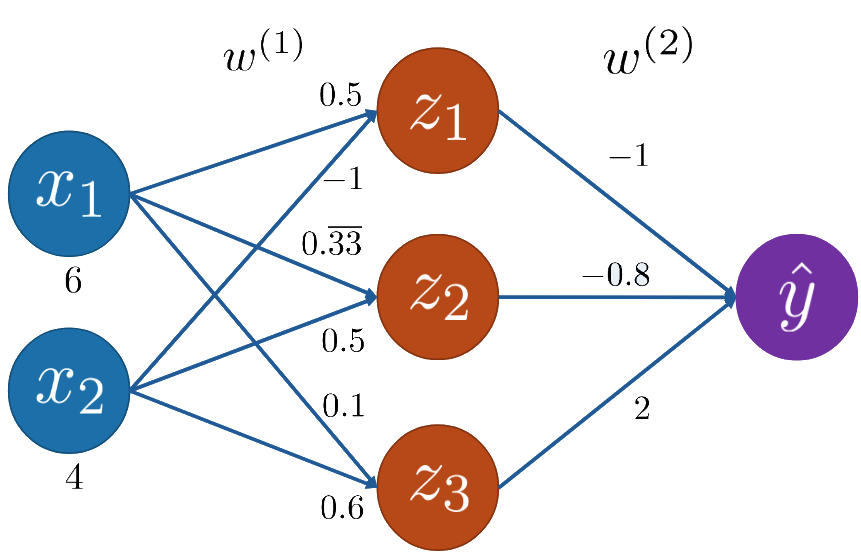
\includegraphics[width=0.5\textwidth]{Pics/11/PredictionNN.png}
\end{figure}

From this we can calculate $z$:

\begin{csmb*}
    $\begin{array}{l}
        z_1 = g\left(w_{0,1}^1 + \sum_{j=1}^{2} x_j \cdot w_{j,1}^1\right) = g\left(x_1w_{1,1}^1 + x_2w_{2,1}^1\right) = g\left(3 + (-4)\right) = g(-1)\\
        z_2 = g\left(2+2\right) = g(4)\\
        z_3 = g\left(0.6 + 2.4\right) = g(3)\\
    \end{array}$
\end{csmb*}

For the activation function $g$ we use the sigmoid function: \inlmathbox{$g(x) = \frac{1}{1 + e^{-x}}$}

This yields $z_1 = 0.26, z_2 = 0.98, z_3 = 0.95$.

To get the prediction $\hat{y}$ we need to calculate the output activation:

\begin{csmb*}
    $\begin{array}{r l}
        \hat{y} &= \sigma\left(w_{0,1}^2 + \sum_{j=1}^{3} z_j \cdot w_{j,i}^2\right)\\ 
        &= \sigma\left(w_{0,1}^2 + z_1w_{1,1}^2 + z_2w_{2,1}^2 + z_3w_{3,1}^2\right)\\
        &= \sigma\left((-1)\cdot 0.26 + (-0.8) \cdot 0.98 + 2 \cdot 0.95\right)\\
        &= \sigma(0.856) = 0.7\\
    \end{array}$
\end{csmb*}

With this we can conclude, that according to our model, the student has a 70\% chance of passing the exam.

\subsection{Backpropagation}
Assume different weight than in the example above so that $\hat{y} = 0.14$.

\begin{minipage}
    [t]{0.5\textwidth}
    \begin{defbox}
        [Quantifying Loss]
        \begin{csmb*}
            $\mathcal{L}\left(f(x^i; \theta), y^i\right)$ 
        \end{csmb*}
    
        Describes the cost of incorrect predictions.
    \end{defbox}
\end{minipage}
\begin{minipage}
    [t]{0.5\textwidth}
    \begin{defbox}
        [Empirical Loss]
        \begin{csmb*}
            $J(\theta) = \frac{1}{n} \sum_{i=1}^{n} \mathcal{L}\left(f(x^i; \theta), y^i\right)$
        \end{csmb*}
    
        Measures the total loss over the dataset. Also known as \defc{objective function, cost function or emprical risk}.
    \end{defbox}
\end{minipage}

Our goal is to \defc{minimize the empirical loss}:

\begin{csmb*}
    $\theta^{\ast} = \underset{\theta}{\arg\min}\space\space J(\theta)$
\end{csmb*}

$\theta^{\ast}$ is the weight setting where the empirical loss is minimized.

This can be done using \defc{Gradient descent}, as the \defc{Weight space} is a N-dimensional space where N ist the total number of weights. 

Algorithm:
\begin{enumerate}
    \item Initialize weights randomly
    \item Loop until convergence
    \begin{itemize}
        \item Compute gradient $\displaystyle \frac{\partial J(\theta)}{\partial \theta}$
        \item Update weights $\theta \leftarrow \theta - \alpha \frac{\partial J(\theta)}{\partial \theta}$ (with $\alpha$ learning rate)
    \end{itemize}
    \item Return weights
\end{enumerate}

\begin{defbox}
    [How to compute $\displaystyle \frac{\partial J(\theta)}{\partial \theta}$]
    Main Question: How much do the weights affect the outcome i.e. the final loss?

    Using the chain rule we can describe the problem as:

    \begin{minipage}
        [t]{0.5\textwidth}
        \centering
        \begin{csmb*}
            $\frac{\partial J(\theta)}{\partial w_2} = \frac{\partial J(\hat{y})} \cdot \frac{\partial \hat{y}}{\partial w_2}$
        \end{csmb*}
    \end{minipage}
    \begin{minipage}
        [t]{0.5\textwidth}
        \centering
        \begin{csmb*}
            $\frac{\partial J(\theta)}{\partial w_1} = \frac{\partial J(\theta)}{\partial \hat{y}} \cdot \frac{\partial \hat{y}}{\partial z_1}\cdot \frac{\partial z_1}{\partial w_1}$
        \end{csmb*}
    \end{minipage}

    We can repeat this for every weight in the network using the gradient from later layers: Propogate the error back to all nodes, through the network.

    \begin{center}
        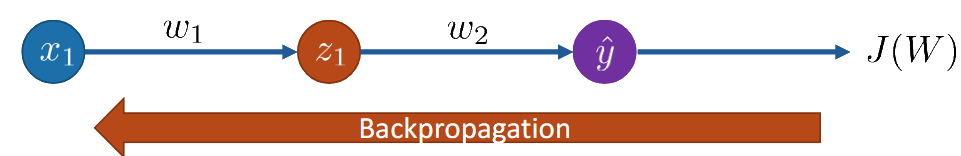
\includegraphics[width=0.7\textwidth]{Pics/11/Backpropagation.png}
    \end{center}
\end{defbox}

\subsubsection*{Example}
\begin{figure}
    [H]
    \centering
    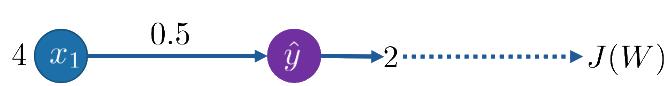
\includegraphics[width=0.6\textwidth]{Pics/11/BackpropagationExample.png}
\end{figure}

Given $g = ReLU(x) = \max(0,x),x_1 = 4,y = 1, \hat{y} = 2, \mathcal{L} = (\hat{y} - y)^2, J(\theta) = \mathcal{L}$

\begin{defbox}
    [ReLU: Rectified Linear Unit]
    If x is greater than 0 return x else return 0.
\end{defbox}

Goal: $\displaystyle \frac{\partial J(\theta)}{\partial w_1} = \frac{\partial J(\theta)}{\partial \hat{y}} \cdot \frac{\partial \hat{y}}{\partial w_1}$

\begin{mathbox*}
    \begin{enumerate}
        \item $\displaystyle \frac{\partial J(\theta)}{\partial \hat{y}} = 2(\hat{y} - y) = 2(2 - 1) = 2$ (Power rule)
        \item $\frac{\partial \hat{y}}{\partial w_1} = ReLU'\left(w_0 + \sum_{i=1}^{n} w_ix_i\right) \cdot x_1 = 1 \cdot 4 = 4$
        \item $\displaystyle \frac{\partial J(\theta)}{\partial w_1} = \frac{\partial J(\theta)}{\partial \hat{y}} \cdot \frac{\partial \hat{y}}{\partial w_1} = 2 \cdot 4 = 8$
    \end{enumerate}

    Now we also need to update the weights $\theta = \theta - \alpha \frac{\partial J(\theta)}{\partial \theta}$ (assume learning rate $\alpha = 0.05$):

    $\theta_{\text{new}} = \theta_{\text{current}} - \alpha \frac{\partial J(\theta)}{\partial \theta}$\\
    $\theta_{\text{new}} = 0.5 - 0.05 \cdot 8 = 0.1$
\end{mathbox*}

Loss function in general are hard to optimize as its difficult to find a global minimum.

\textbf{Basic Idea:}\\
Change weight into the direction of the steepest descent of the error function given a step size - This step size is called the \defc{learning rate $\alpha$}, but finding a good value is hard.

\begin{figure}
    [H]
    \centering
    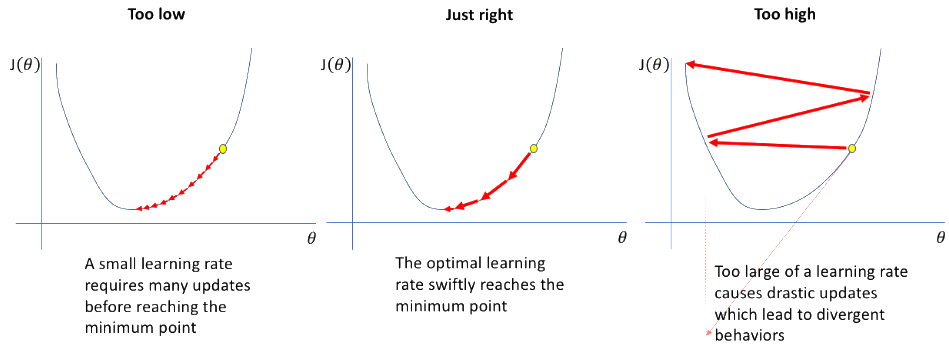
\includegraphics[width=\textwidth]{Pics/11/LearningRate.png}
\end{figure}
\end{document}